\section{Reinforcement Learning}

\begin{frame}[fragile]{Machine Learning}
\begin{itemize}
  \item Supervised Learning
    \begin{itemize}
      \item Classification
      \item Regression
    \end{itemize}
  \item Unsupervised Learning
    \begin{itemize}
      \item Clustering
      \item ...
    \end{itemize}
  \item \alert{Reinforcement Learning}
\end{itemize}
\end{frame}

\begin{frame}[fragile]{Agent Environment}
\tikzstyle{block} = [rectangle, draw,
text width=8em, text centered, rounded corners, minimum height=4em]
\tikzstyle{line} = [draw, -latex]
\begin{figure}
    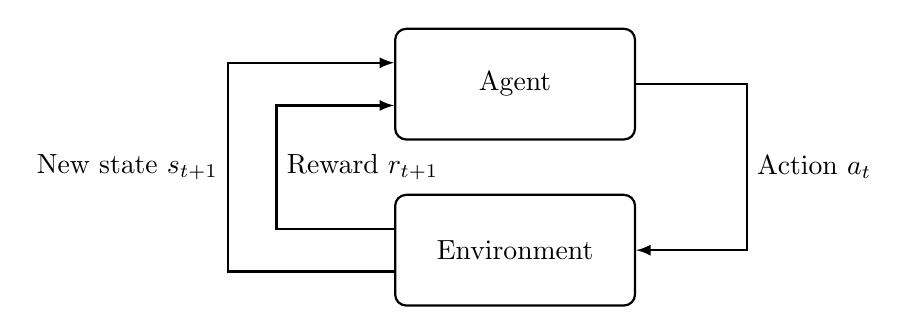
\begin{tikzpicture}[node distance = 6em, auto, thick]
        \node [block] (Agent) {Agent};
        \node [block, below of=Agent] (Environment) {Environment};

        \path [line] (Agent.0) --++ (4em,0em) |- node [near start]{Action $a_t$} (Environment.0);
        \path [line] (Environment.190) --++ (-6em,0em) |- node [near start] {New state  $s_{t+1}$} (Agent.170);
        \path [line] (Environment.170) --++ (-4.25em,0em) |- node [near start, right] {Reward $r_{t+1}$} (Agent.190);
    \end{tikzpicture}
    \caption{Agent environment interface}
\end{figure}
\end{frame}

\begin{frame}[fragile]{Markov Decission Process}
   \textbf{\textsc{Markov Decission Process}} is defined by  quatuple  $\left\langle \mathcal{S},\, \mathcal{P},\, \mathcal{R} ,\ \mathcal{A} \right\rangle $
\begin{itemize}
    \item $\mathcal{S}$, a set of states
    \item  $\mathcal{P}$, a state transition matrix defining the probabilities of some possible next state $s'$ given any state $s$
          $\mathcal{P}^a_{ss'}= \mathbb{P} [ S_{t+1}=s'|S_{t}=s , A_t = a ]$
    \item a reward function $\mathcal{R}^a_s=\mathbb{E}[R_{t+1}|S_{t}=s , A_t = a ]$
    \item $\mathcal{A}$, a set of actions
\end{itemize}
\end{frame}

\begin{frame}[fragile]{Policy}
\begin{itemize}
    \item specifies agent's behaviour
    \item mapping of state to action
\end{itemize}
\begin{equation*}
    \pi(s)= a
\end{equation*}
\begin{equation*}
    \mathbb{P}(a|s)= \pi(a|s)
\end{equation*}
\end{frame}

\begin{frame}[fragile]{Markov Property}
    \begin{columns}
        \column{0.5\textwidth}
        \begin{itemize}
            \item The future is conditionally independent of the past given the presence
            \item implies memorylessnes 
        \end{itemize}
        \column{0.5\textwidth}
\begin{equation*}
    \mathbb{P}[S_{t+1}|S_{1},\ldots,S_{t}]=\mathbb{P}[S_{t+1}|S_{t}] 
\end{equation*}
\end{columns}
\end{frame}

\begin{frame}[fragile]{Taxonomy of RL}
 \begin{figure}[h]
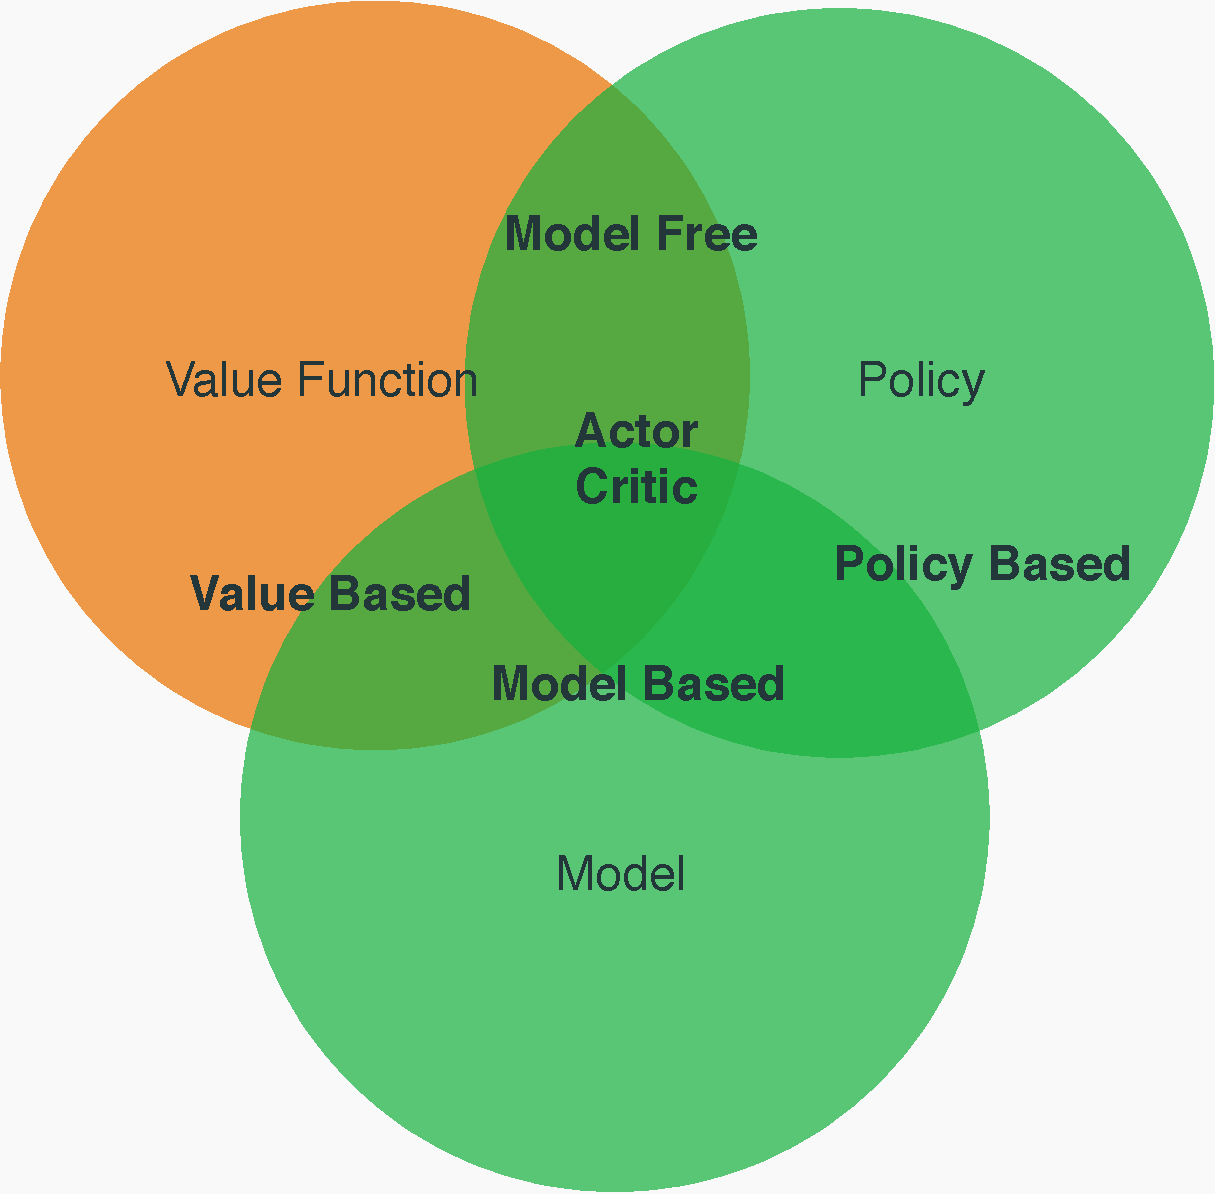
\includegraphics[width=0.7\textwidth]{taxovennxml}
\end{figure} 
\end{frame}

\begin{frame}{Value Function}
    Expected return
      \begin{itemize}
        \item from state $s$ and  action $a$ 
        \item given policy $\pi$

      \begin{equation*}
        Q^{\pi}(s,a)=\E [r_{t+1}+ \gamma r_{t+2}+\gamma^2 r_{t+3}+\ldots|s,a]
      \end{equation*}

      \item decomposable into
      \begin{equation*}
        Q^{\pi}(s,a)=\E [r+\gamma Q^{\pi}(s', a')|s,a]
      \end{equation*}
      \end{itemize}
\end{frame}

\begin{frame}{Optimal Value Function}
      \begin{itemize}
        \item optimal value function

      \begin{equation*}
        Q^{*}(s,a)=\max_{\pi} Q^{\pi}(s,a)=Q^{\pi^*}(s,a)
      \end{equation*}

      \item optimal policy

      \begin{equation*}
        \pi^{*}(s)=\argmax_{a}Q^*(s,a)
      \end{equation*}

    \item decomposition into

      \begin{equation*}
        Q^{*}(s,a)=\E_{s'}[r+\gamma \max_{a'}Q^{*}(s',a')|s,a]
      \end{equation*}

      \end{itemize}
\end{frame}

\begin{frame}{TD Learning}
          \metroset{block=fill}

Off Policy learning 
      \begin{block}{Q-learning}
        \begin{equation*}
            Q(S_t,A_t)\gets Q(S_t,A_t)+\alpha[\underbrace{\underbrace{R_{t+1}+ \gamma \max_a Q(s_{t+1},a)}_{\text{target}}-\underbrace{Q(S_t,A_t)}_{\text{prediction}})}_{\text{TD-Error}}]
        \end{equation*}
      \end{block}

On Policy learning
      \begin{block}{Sarsa}
        \begin{equation*}
            Q(S_t,A_t)\gets Q(S_t,A_t)+\alpha[R_{t+1}+ \gamma Q(s_{t+1},A_{t+1})-Q(S_t,A_t))]
        \end{equation*}
      \end{block}

\end{frame}
\begin{frame}{Backup Diagrams}
  \begin{figure}
  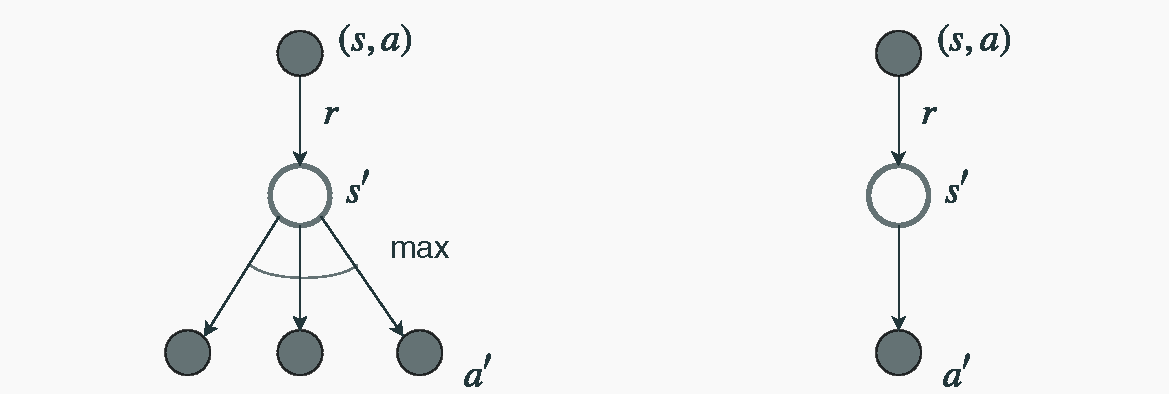
\includegraphics[width=\textwidth]{qlearningsarsagrey}
  \caption{backup diagram for Q-learning and Sarsa}
  \end{figure}
\end{frame}
\begin{frame}{Q-learning}
      \begin{algorithmic}[0]
        \State Initialize $Q(s, a)$ arbitrarily
        \State Initialize  $S$
        \Repeat
        \State Choose $A$ from $S$ using policy derived from $Q$
        \State Take action $A$ observe $R,\,S'$
        \State Choose $A'$ from $S'$ using policy derived from $Q$
        \State $Q(S,\,A) \gets Q(SA)+\alpha[R+\gamma\max_{a} Q(S',\,a)-Q(S\,A)]$
        \State $S\gets S'$
        \Until $S$ is terminal
    \end{algorithmic}
  \end{frame}
\begin{frame}[standout]
  Demo
\end{frame}

